\section{Theoretical Framework}

In order to thoroughly understand the aim and subject of the research, it is important to explore different existing solutions and literature. Therefore, the subjects that will be discussed in the  following theoretical framework are Cloud Streaming/Cloud Computing and Virtual Reality. Within this theoretical framework, definitions of the subjects will be given as well as current insights into these subjects. The topics reflect knowledge needed to understand the problem space. Together all of the topics make up the 360 scan.

\subsection{Cloud Streaming/Cloud Computing}

\subsubsection{Definition}
According to Armbrust et al. (2010) Cloud computing is defined as follows: 
"Cloud computing refers to both the applications delivered as services over the Internet and the hardware and systems software in the data centers that provide those services." \parencite[]{aviewoncc}
We can then further define Cloud streaming as the applications that are delivered over the internet as a service.

\subsubsection{Existing Solutions and Technology}
Several commercial gaming Cloud streaming services already exist, such as Google Stadia \parencite{stadia}, XBox XCloud \parencite{xcloud} and Nvidia GeForceNow \parencite{geforcenow}. These applications deliver conventional games from a powerful computer in a server to the client device at home. Despite initial setbacks, cloud streaming is now a mainstream technology. The start of 2020 also saw the first experimental cloud \acrshort{vr} streaming development kits, such as Nvidia's CloudXR \parencite{cloudxr}. However no commercial cloud VR streaming services exists. at the time of writing. There is also a variety of Infrastructure\hyp{}as\hyp{}a\hyp{}service (IaaS) platforms, such as Amazon's AWS \parencite{aws}, Microsoft's Azure \parencite{azure} and Google's Cloud Platform \parencite{gcp}, that provide generic computing power and storage in a cloud computing/streaming context. For more information about these applications and technologies, please refer to the \hyperref[sec:lit]{Literature Analysis}.

\subsubsection{System Architecture (for a cloud system)}
\begin{figure}[h]
\caption{Cloud Server, Remote Edge, Local Edge visualized \parencite{wlanvr}}
\label{fig:arch1}
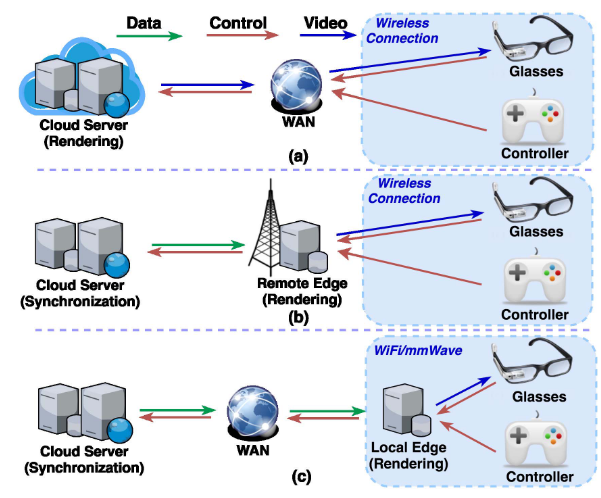
\includegraphics[scale=0.45]{Architectures1}
\end{figure}

\begin{figure}[!htbp]
\caption{Example System Architecture}
\label{fig:sysarch}
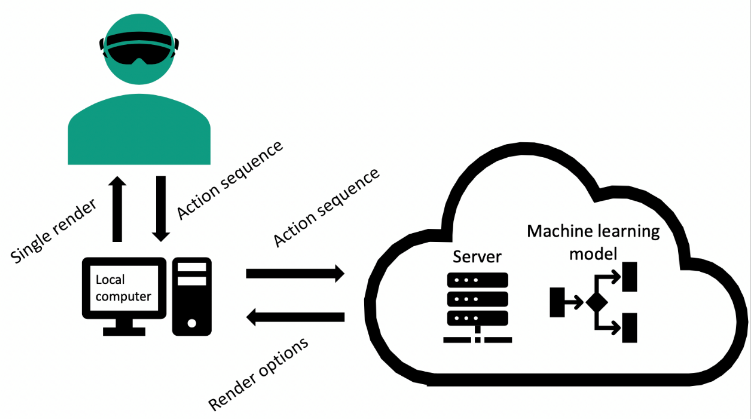
\includegraphics[scale=0.45]{SimpleArchitecture}
\end{figure}

One of the main considerations when designing a cloud \acrshort{vr} streaming application is the decision to either use a Cloud, Remote Edge or Local Edge computing device for the rendering of the frames (See \hyperref[fig:arch1]{Figure 1} and \cite{wlanvr}):
\begin{itemize}
\item A cloud server renders the \acrfull{fov} (current view) remotely and streams the corresponding video to the user’s \acrfull{hmd}. 
\item A Remote Edge sever recieves multiple views that are rendered remotely on cloud servers, stitches them together to a 360-degree video, and streams the video to the user’s \acrshort{hmd}
\item A Local Edge server recieves compressed models as well as textures, renders it locally and streams the video to the user’s \acrshort{hmd}.
\end{itemize} 

Since this project is focused on a cloud streaming, we will disregard the local edge approach an instead focus on solutions that use a cloud server or remote edge server for rendering. An example architecture of such a solution can be seen in \hyperref[fig:sysarch]{Figure 2}.
\subsubsection{Latency}
The most important metric for a system architecture is the latency between the user input, such as movement of the \acrshort{hmd}, and the updated frame appearing on the users display. Recent measurements of  cloud gaming services measure this latency at between 135 and 240 \acrshort{ms} \parencite{lagmeasure}. This is acceptable for most games, except maybe high intensity reaction games. \acrshort{vr} unfortunately has severely stricter latency requirements, which are elaborated upon in \hyperref[ssec:vrphy]{the next section}.

\subsection{Virtual Reality}

\subsubsection{Definition}
Early works, such as the 1996 article "Virtual Reality in Scientific Visualizations"  or the 2003 book "Virtual Reality Technology", define Virtual Reality as: "The use of computers and human\hyp{}computer interfaces to create the effect of a three\hyp{}dimensional world containing interactive objects with a strong sense of three\hyp{}dimensional presence."\parencite{vrsv} or "A Simulation in which computer graphics is used to create a realistic looking world. Moreover, the synthetic world is not static, but responds to the users input. This defines a key feature of Virtual Reality, \textit{real\hyp{}time interactivity}" \parencite{vrtech}.

\subsubsection{Physical Constraints}
\label{ssec:vrphy}
As mentioned before, when developing a \acrshort{vr} application, there are a few physical constraints that developers need to be aware of. The most important threshold to know is the 20 \acrshort{ms} \acrfull{mtp} delay. Upon input from the \acrfull{hmd}, the developer has to display a new rendered image within an average of 20 \acrshort{ms} to avoid motion sickness for users. The more this threshold can be undercut, the better the chances to have an acceptable gameplay experience without motion sickness. Interaction input, such as the input from the controllers, can safely be processed at delays of $>$100 \acrshort{ms} without any negative repercussions in terms of \acrfull{ux}. For more information, please refer to the \hyperref[sec:lit]{Literature Analysis}.